\section{Metodi e Modelli}

\subsection{Modello ad Agente}

Il modello ad agente implementato pone l'accento sull'idea di avere
un controllo granulare sulla localizzazione dei possibili 
focolari o punti di interesse durante il ciclo di vita di una pandemia.
Per modellare uno spazio simile e' stato utilizzato uno \textbf{spazio discreto 
a grafo}. 

L'idea e' quella di rappresentare differenti punti di interesse astratti dal
livello di dettaglio che si vuole andare a modellare, andando a generalizzare
uno scenario tipo nel quale N agenti si muovono all'interno di una rete 
(in questo caso un grafo) e con questo monitorare diversi tipologie di interventi
e il loro grado di successo nella lotta contro una possibile pandemia.

La struttura offerta dal framework \textbf{Agents.jl} e' quella di uno 
spazio \emph{GraphSpace} in coppia con il relativo tipo di agente di default
\emph{GraphAgent}. Non vi e' alcuna differenza tra la tipologia GraphAgent e 
ad esempio l'interfaccia AbstractAgent, in quanto il primo deriva dal secondo. 
Tuttavia GraphAgent ha gia' al suo interno tutti gli attributi utili per 
gestire un agente all'interno di uno spazio a grafo, lasciando al programmatore una
preoccupazione in meno. 

\subsubsection*{Agente}
\begin{minipage}{\linewidth}
    \centering
    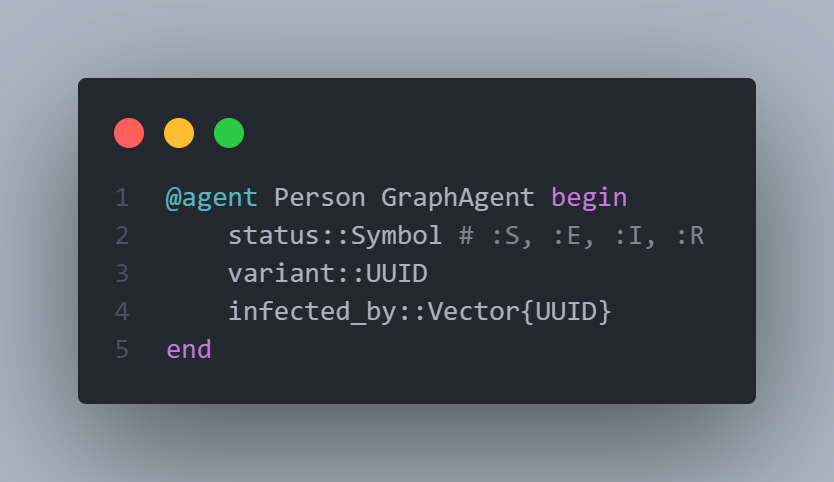
\includegraphics[width=\textwidth]{img/agent_code.png}
    \captionof{figure}{Codice Agente}
    \label{fig:Agent_code}
\end{minipage}

Come e' possibile vedere dalla Figura \ref{fig:Agent_code}, il codice che si occupa
di creare l'agente e' estremamente semplice. Al suo interno troviamo tutto quello che 
un agente deve sapere per poter agire in maniera corretta all'interno dell'ambiente. 
Essendo che l'agente \emph{Person} deriva dall'agente GraphAgent, questo eredita 
automaticamente i campi fondamentali \textbf{pos} e \textbf{id}, i quali serviranno 
per riconoscere la posizione all'interno del grafo dell'agente e distinguere l'agente 
dagli altri.

I campi principali sono:
\begin{itemize}
	\item status: e' un campo di tipo \textbf{Symbol} che rappresenta 
	lo stato di un determinato agente in un preciso momento del tempo. 
	Questo stato puo' mutare nel tempo ed e' strettamente correlato a 
	tutti e soli gli stati che un individuo puo' assumere all'interno di
	un modello matematico di tipologia \textbf{SEIR}
	\item variant:  e' un campo di tipo \textbf{UUID} (Universally Unique ID)
	che rappresenta un identificatore univoco associato ad una delle possibili
	varianti dell'agente patogeno attualmente in circolazione. Questo attributo 
	serve principalmente a gestire la possibilita' di non avere una completa
	immunita' dopo aver contratto e aver debellato il virus dal proprio sistema 
	immunitario, rendendo gli individui identificati come \textbf{:R} 
	passibili di reinfezione
	\item infected by: e' un campo di tipo \textbf{Vector} che rappresenta 
	quali varianti sono state contratte dall'agente. Un agente non puo' piu'
	essere infettato da queste varianti. Questo approccio e' stato ideato per 
	la modellazione di un vaccino, il quale non e' detto che copra tutte le
	varianti che sono uscite, o comunque non e' detto che, pur coprendo tutte le
	varianti conosciute copra anche quelle non conosciute.
\end{itemize}

Utilizzare la macro \textbf{@agent} e' il modo che viene incentivato dal linguaggio, in quanto
permette di creare un agente da un super tipo come AbstractAgent e permette di avere 
gia' inclusi tutti i campi necessari. Inoltre, utilizzando questa \textbf{macro} e' 
possibile includere tutti i campi di un altro agente, dovendo solamente specificare quelli 
nuovi.

\subsubsection*{Spazio e Modello}
Lo spazio e' di tipo GraphSpace e viene definito direttamente in 
fase di creazione del modello. 

\begin{minipage}{\linewidth}
    \centering
    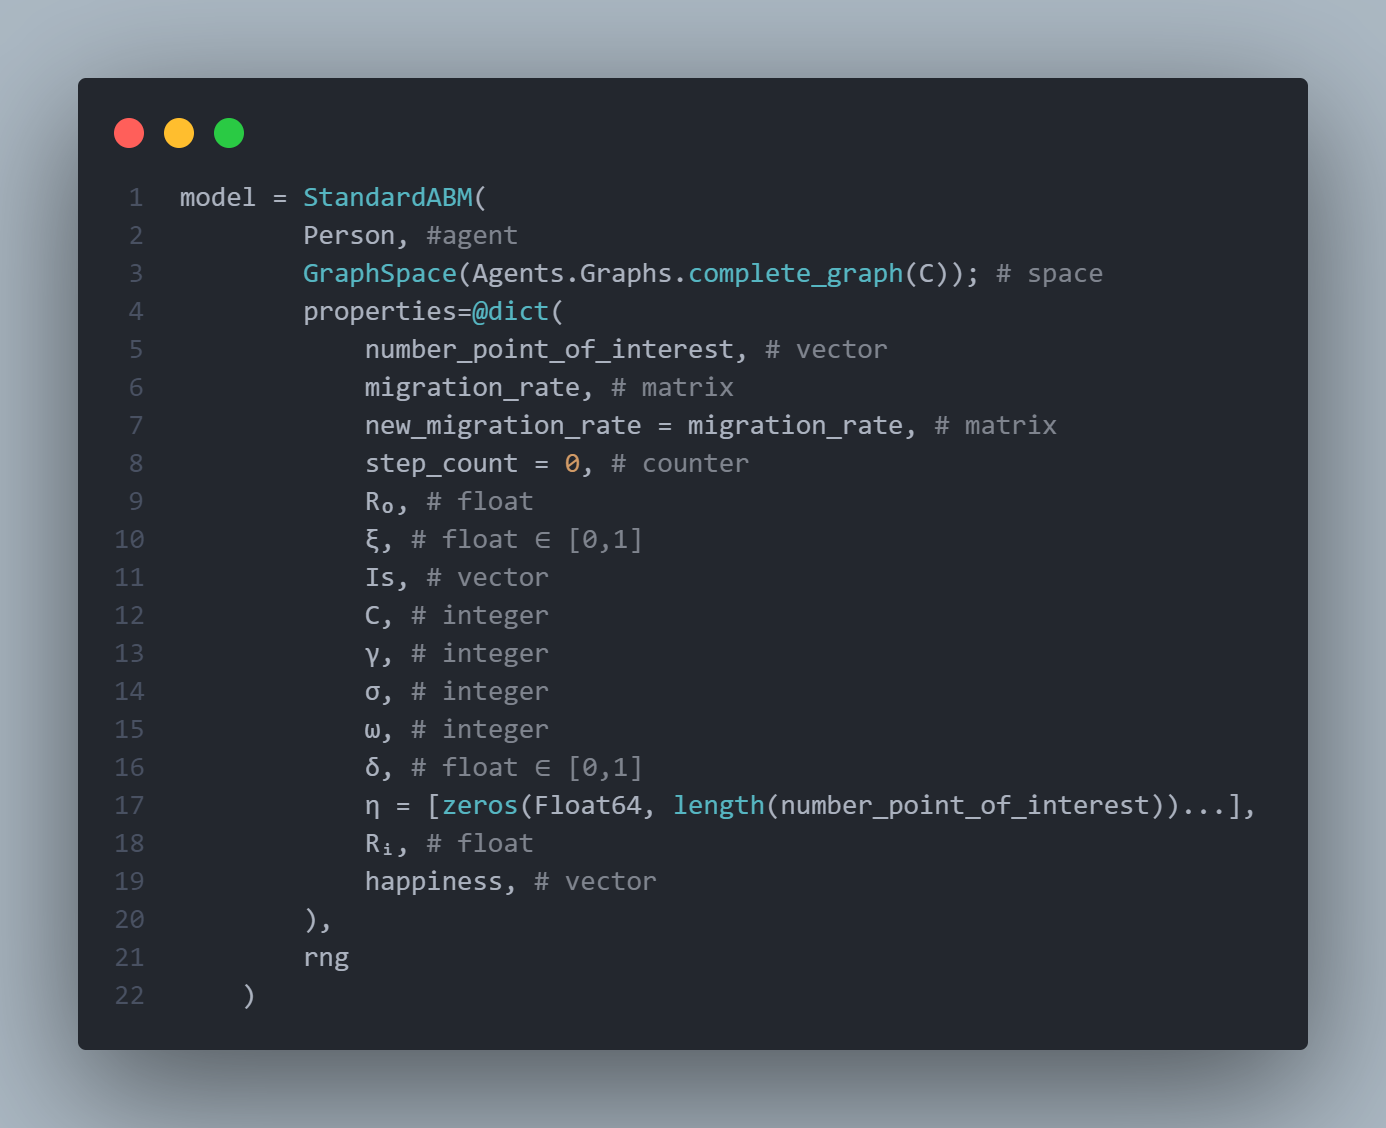
\includegraphics[width=\textwidth]{img/model_code.png}
    \captionof{figure}{Codice Modello}
    \label{fig:model_code}
\end{minipage}

In questo caso come si puo' osservare dalla Figura \ref{fig:model_code}, lo spazio 
e' un \emph{grafo completo} con C nodi. I nodi corrispondono ai punti di interesse del 
grafo. Per dettagliare maggiormente questo spazio altrimenti scarno, vengono definite delle 
\emph{proprieta' spaziali} del modello, ovvero proprieta' che ci sono sempre e ovunque. 
Queste proprieta' possono essere divise in due macro categorie: proprieta' dei punti di interesse
e proprieta' della pandemia.

Le proprieta' dei punti di interesse sono le seguenti:
\begin{itemize}
	\item number point of interest: e' di tipo \textbf{Vector} e rappresenta il numero di agenti 
	che quel determinato nodo puo' contenere. Gli elementi all'interno di questo vettore vengono 
	determinati tramite una funzione esponenziale.
	\item migration rate: e' di tipo \textbf{Matrix} e rappresenta una matrice di transizione tra i 
	vari nodi del grafo. Questa matrice di transizione codifica la probabilita' di un agente di spostarsi
	dal suo nodo ad un qualsiasi altro nodo presente. Essendo il grafo di tipo completo, ogni nodo 
	e' collegato a tutti gli altri, tuttavia non tutti i collegamenti sono equamente probabili.
	La matrice infatti tiene in considerazione la probabilita' di un agente di spostarsi piu' 
	facilmente verso un nodo popoloso, piuttosto che verso uno che non lo e', questo a mimica degli 
	spostamenti umani.

	\begin{minipage}{\linewidth}
		\centering
		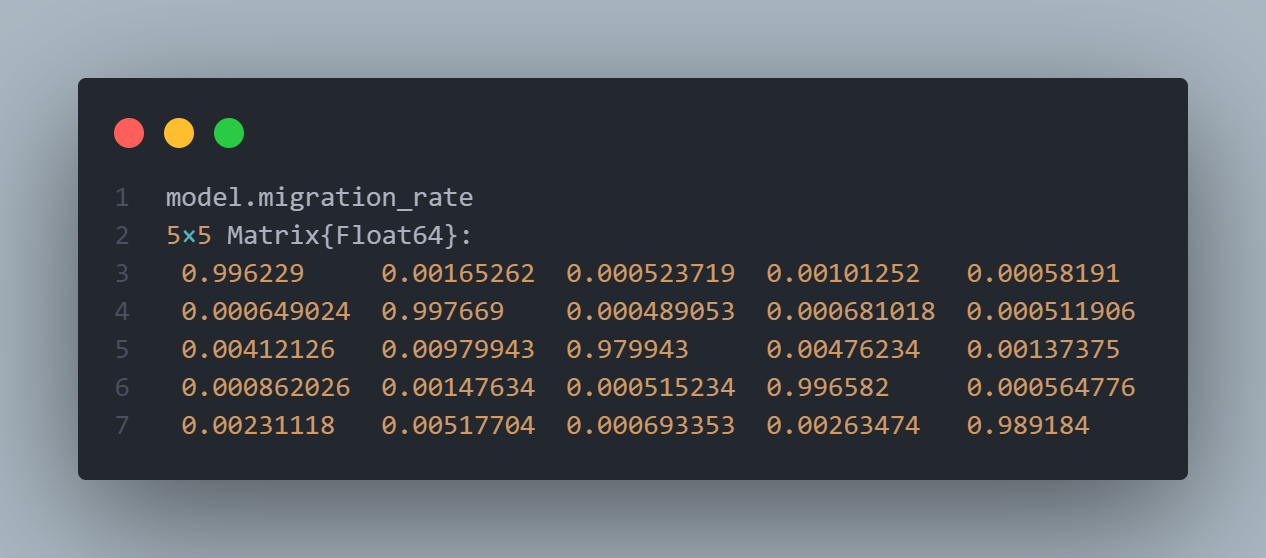
\includegraphics[width=\textwidth]{img/travel_rate.png}
		\captionof{figure}{Esempio di matrice di transizione}
		\label{fig:migration_matrix}
	\end{minipage}

	\item Is: e' di tipo \textbf{Vector} e rappresenta il vettore degli infetti iniziali.
	Generalmente viene inizializzato randomicamente nella posizione dei nodi, ma fisso nel numero
	di infetti ovvero con I = 1. 
	\item $\eta$: e' di tipo \textbf{Vector} e rappresenta il vettore delle contromisure implementate.
	L'esperienza della pandemia ci ha insegnato che non sempre una contromisura generalizzata e' qualcosa
	che funziona, alle volte e' giusto trattare in maniera locale il problema, applicando contromisure mirate
	alla tipologia di esigenza locale. Questo vettore raccoglie quindi le contromisure associate ad ogni 
	nodo del grafo. Una contromisura e' un valore $\in [0,1]$ che identifica l'efficacia della contromisure applicate.
	La sfida e' comprendere in che modo una contromisura impatti sulla diffusione della pandemia.
	\item happiness: e' di tipo \textbf{Vector} e rappresenta il vettore della felicita' della popolazione 
	di un determinato nodo. Questo vettore contiene valori $\in [-1,1]$. Questo parametro e' stato inserito 
	per evitare una caduta in una strategia funzionale ma insostenibile. Se l'obiettivo di un controllore 
	e' quello di minimizzare il numero di infetti (e morti), la scelta piu' ragionevole (non dovendo tenere 
	in conto di null'altro), e' quella di applicare un lockdown generalizzato a tutta la popolazione. 
	Terminato il periodo di vita del virus si e' risolta la crisi pandemica. Questa soluzione e' pero'
	\textbf{umanamente insostenibile}. Da qui un termine aggiuntivo che il controllore deve bilanciare, 
	ovvero la felicita' della popolazione. Infatti questo termine deve essere massimizzato, e dipende 
	principalmente dal termine $\eta$.
\end{itemize}

Le proprieta' della pandemia sono invece:
\begin{itemize}
	\item $R_0$: e' di tipo \textbf{Float64} e rappresenta l'indice di infettivita' di un virus
	\item $\gamma$: e' di tipo \textbf{Int} e rappresenta il numero di giorni dopo di cui un paziente
	che ha contratto il virus puo' considerarsi guarito
	\item $\sigma$: e' di tipo \textbf{Int} e rappresenta il numero di giorni per cui un agente dopo essere
	stato infettato viene considerato \emph{esposto}, per cui non ancora in grado di infettare, ma che una 
	volta terminato questo periodo diventera' infettivo
	\item $\omega$: e' di tipo \textbf{Int} e rappresenta il numero di giorni per cui un agente e' considerato
	immune alla malattia dopo essere guarito da essa
	\item $\delta$: e' di tipo \textbf{Float64} e rappresenta la probabilita' di un agente infetto di morire al 
	termine del proprio periodo di infettivita' ($\gamma$).
	\item $\xi$: e' di tipo \textbf{Float64} $\in [0,1]$ e rappresenta, una volta che e' stato introdotto un vaccino come metodo 
	di prevenzione controil virus, il rateo di individui S che che possono essere vaccinati, e quindi diventare R,
	al giorno.
	\item $R_i$: e' di tipo \textbf{Float64} e rappresenta l'indice di infettivita' desiderato, che si vuole
	raggiungere per arginare la malattia e fermarne l'avanzata. Generalmente questo valore si attesta al piu' 
	intorno a 1.0
\end{itemize}

\subsubsection*{Funzione di avanzamento agente}
Un agente finche' all'interno di un modello segue ciclicamente il comportamento
riportato in figura \ref{fig:agent_behaviour}

\begin{minipage}{\linewidth}
	\centering
	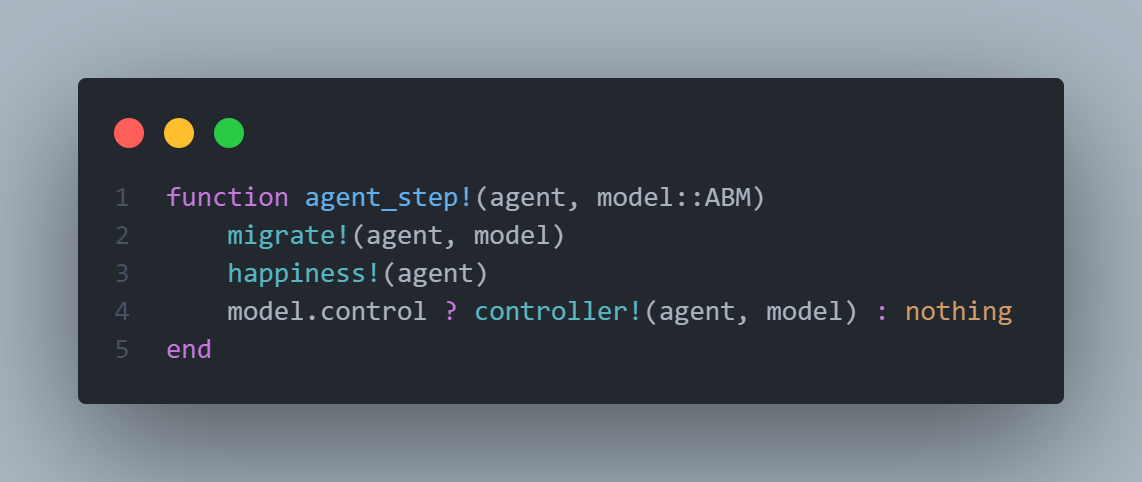
\includegraphics[width=\textwidth]{img/agent_behaviour.png}
	\captionof{figure}{Comportamento agente}
	\label{fig:agent_behaviour}
\end{minipage}

Durante la funzione di avanzamento un agente segue un insieme di regole, che dettano
un comportamento semplice ma completo. Un agente ha il compito di provare a spostarsi di 
nodo, passando da quello attuale ad uno dei molteplici collegati; la scelta del nodo e' 
casuale ma la sua trnasizione dipende dalla matrice di transizione definita precedentemente.
Successivamente l'agente ha il compito di fare da veicolo per le infezioni \textbf{sse} 
il suo stato e' infetto, altrimenti non e' necessario che venga effettuato questo punto.
Infine il compito di un agente e' quello di aggiornare il proprio stato passando potenzialmente
da quello attuale ad uno nuovo; questo implica che e' possibile che un agente venga rimosso 
totalmente dal modello se dovesse morire.

La funzione di trasmissione basa il proprio funzionamento sull' \emph{assunzione} che il 
numero di contatti di un individuo infetto siano distribuiti seguendo
una \textbf{Poisson} con media il parametro $R_0$. Ogni contatto poi ha la possibilita'
di essere infettato data unicamente da due fattori:
\begin{itemize}
	\item stato dell'agente: solamente un agente con stato S (Suscettibile) puo' essere
	infettato, oppure un agente con stato R (Recovered) che non ha mai contratto la variante
	con cui attualmente e' entrato in contatto
	\item probabilita' di infezione: questo valore e' dato dal rapporto tra le variabili
	$R_0$ e $\gamma$ e indica la probabilita' di un infezione secondaria dato un contatto 
	positivo all'essere infetto
\end{itemize}

\begin{minipage}{\linewidth}
	\centering
	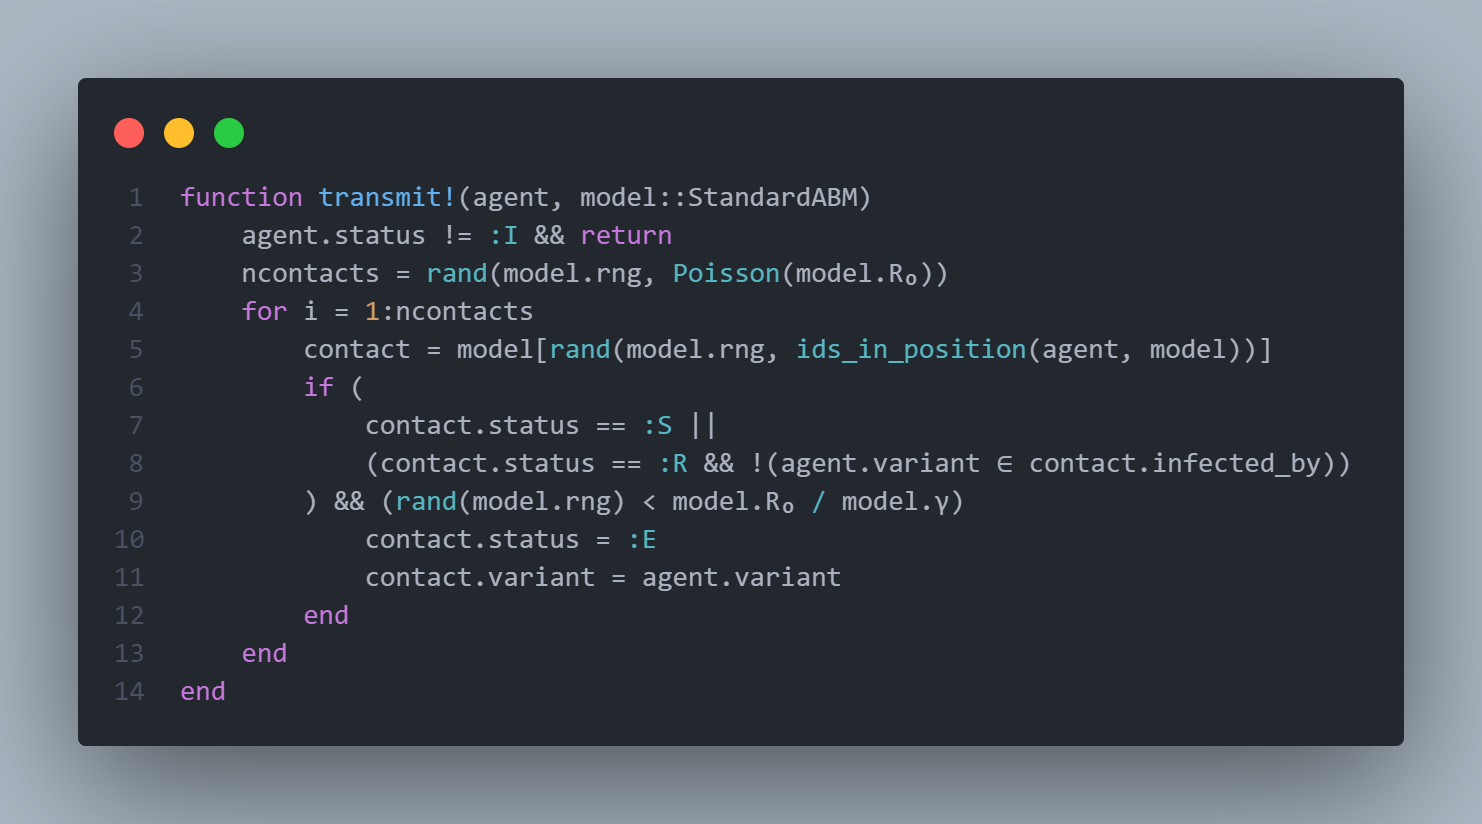
\includegraphics[width=\textwidth]{img/transmit_function.png}
	\captionof{figure}{Funzione di trasmissione}
	\label{fig:transmit_function}
\end{minipage}

La funzione di aggiornamento dello stato degli agenti prende spunto dalla 
funzione di transizione descritta dal modello compartimentale SEIR in figura \ref{fig:SEIRS_model}
tranne che non viene modellata ne la morte naturale ne tantomeno la nascita di nuovi 
agenti all'interno del modello. Viene pero' aggiunta la possibilita' di passare
da uno stato S ad uno R tramite la probabilita' di \textbf{vaccinarsi} definita con il parametro $\xi$.
% TODO: aggiornare figura 

\begin{minipage}{\linewidth}
	\centering
	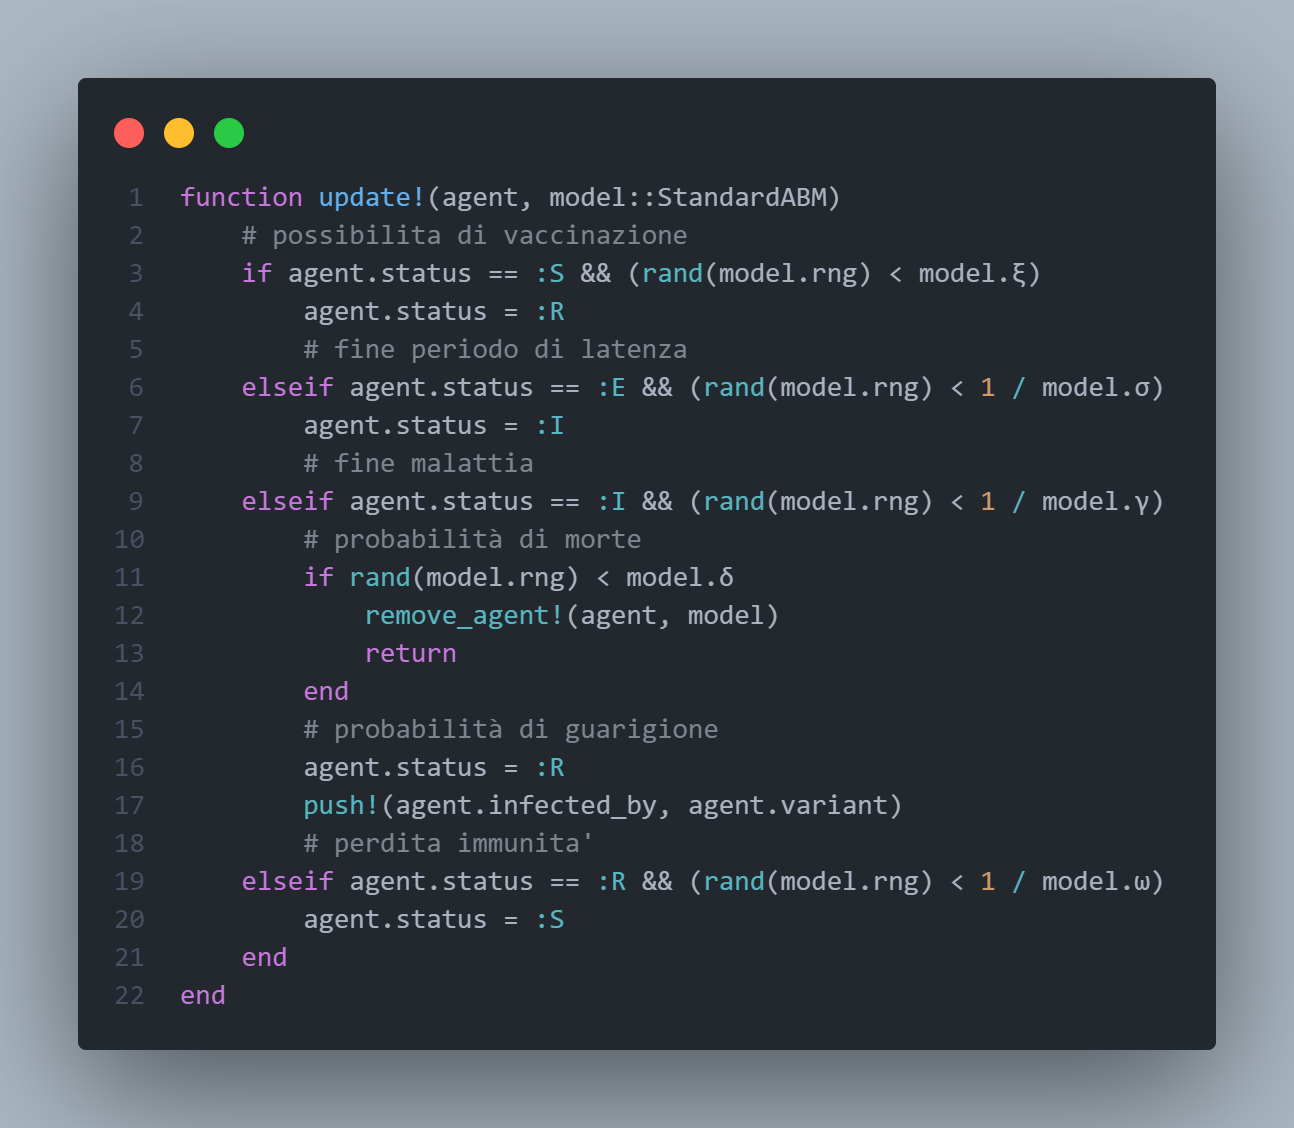
\includegraphics[width=\textwidth]{img/update_function.png}
	\captionof{figure}{Funzione di aggiornamento dello stato di un agente}
	\label{fig:update_agent_function}
\end{minipage}

Come mostrato nella sezione riguardante le proprieta' del modello in figura \ref{fig:model_code},
le proprieta' che descrivono le probabilita' di transizione da uno stato all'altro sono prevalentemente
di tipo \textbf{Int}. Queste pero' vengono poi implicitamente trasformate in tipo \textbf{Float64} 
quando bisogna calcolare la probabilita' di transizion. La scelta di inizializzarle come 
tipo Int e' stata fatta solamente per essere piu' \emph{Human Understandable}.

\subsubsection*{Funzione di avanzamento modello}
Ogni passo di avanzamento del modello segna un passo di avanzamento dell'intero sistema. 
Questo vuol dire che all'interno di un passo del modello vi e' un passo per ogni agente. Di default
il framework Agents.jl effettua prima l'avanzamento degli agenti e successivamente quello del modello.
Questo comportamento puo' essere modificato quando viene chiamata la funzione di \textbf{step!} che 
si occupa di far girare l'intero sistema.

Il modello si occupa ad ogni passo di effettuare tutte quelle operazioni che non sono legate ad un
singolo agente ma che sono legate o alla comunita' di agenti oppure al modello in quanto sistema complesso. 

\begin{minipage}{\linewidth}
	\centering
	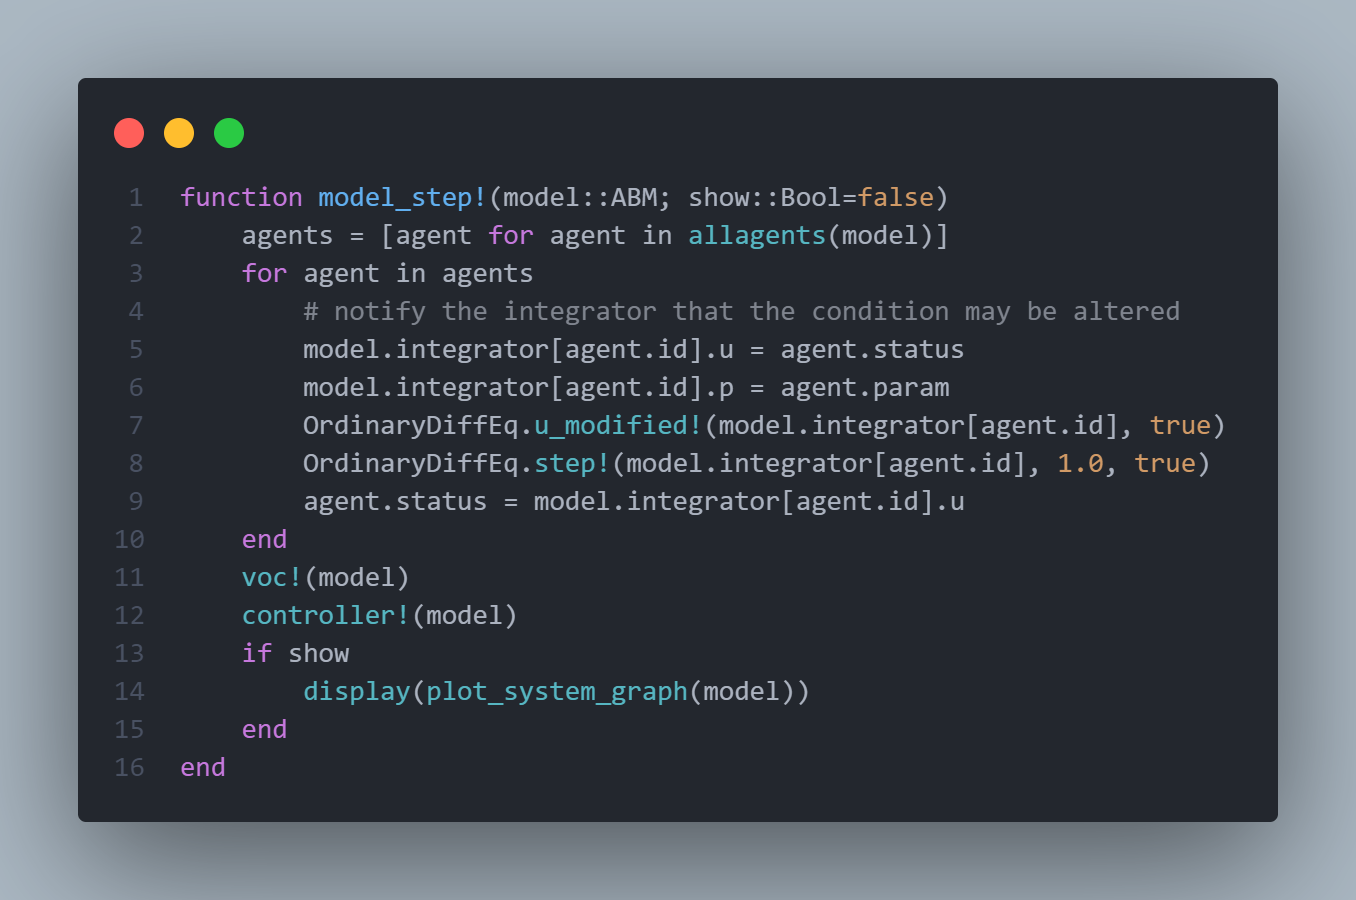
\includegraphics[width=\textwidth]{img/model_step.png}
	\captionof{figure}{Funzione di avanzamento del modello}
	\label{fig:model_step}
\end{minipage}

Come e' possibile osservare dalla figura \ref{fig:model_step}, il sistema si occupa principalmente
di aggiornare la felicita' generale degli agenti, aggiornare l'indice $R_0$ riducendo il suo valore 
in caso in cui sono state prese delle contromisure adeguate, controllare se e' disponibile un vaccino,
generare una nuova \emph{Variant of Concern} (VOC). 

Questa sezione e' quella che piu' presta il fianco ad \emph{assunzioni} riguardo 
il comportamento generale del sistema. Tutte le funzioni sopra descritte si basano su un insieme
piu' o meno nutrito di assunzioni per funzionare correttamente. Questo perche' al momento in cui sto 
redigendo questo documento \today, non sono ancora riuscito ad implementare metodi migliori.

Attualmente la funzione che si occupa di generare la felicita' complessiva di un nodo si basa
sull'utilizzo di una \emph{tangente iperbolica} (tanh) che prende come parametro il valore attuale
di happiness del nodo e lo bilancia con il valore delle contromisure $\eta$ associate e attualmente 
uso. Questo approccio e' sicuramente problematico e fallace per numerosi motivi ma attualmente 
adempie al suo obiettivo. 

\begin{minipage}{\linewidth}
	\centering
	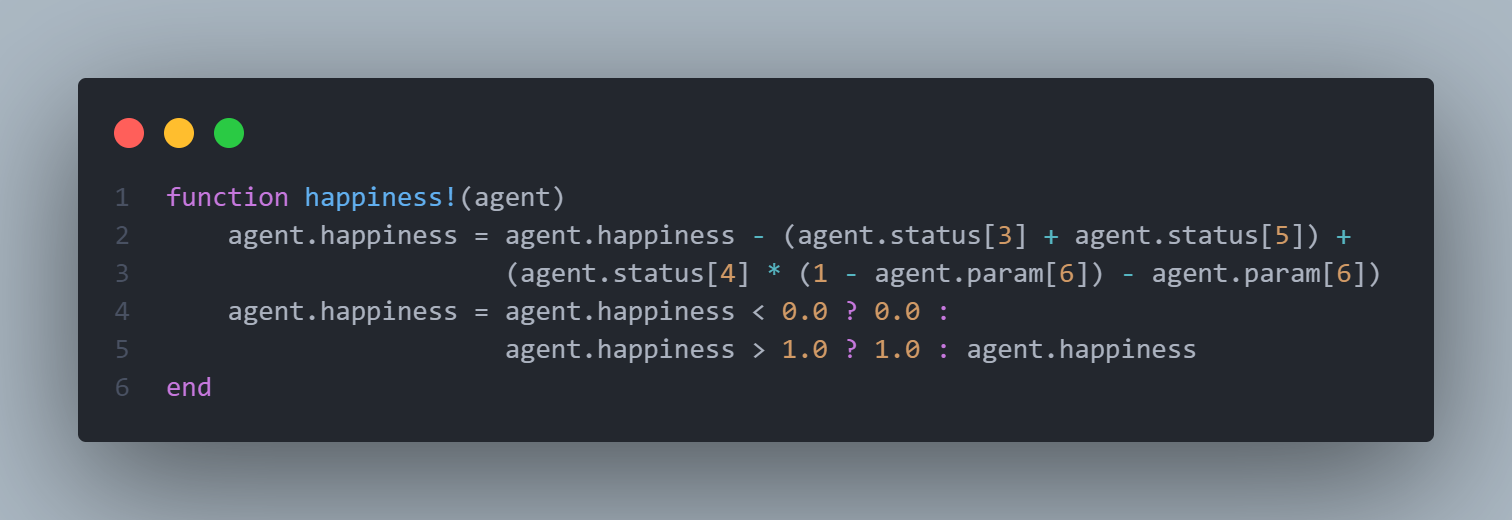
\includegraphics[width=\textwidth]{img/happiness.png}
	\captionof{figure}{Funzione di stima della felicita generale di un nodo del grafo}
	\label{fig:happiness}
\end{minipage}

La funzione di aggiornamento dell'indice $R_0$ in relazione a $\eta$ riduce ad ogni passo 
del modello il valore di $R_0$ proporzionalmente al valore di $\eta$ e del
valore di $R_i$, ovvero il valore atteso di $R_0$ che si vuole ottenere. 

\begin{minipage}{\linewidth}
	\centering
	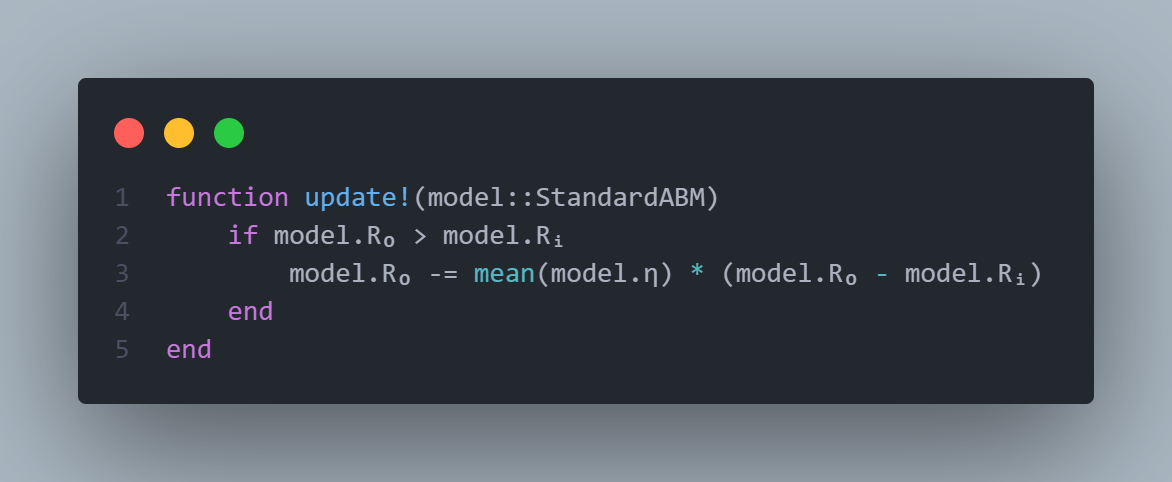
\includegraphics[width=\textwidth]{img/r0_reduction.png}
	\captionof{figure}{Funzione di riduzione $R_0$}
	\label{fig:r0_reduction}
\end{minipage}

Come mostrato in figura \ref{fig:r0_reduction} questo metodo si basa su un aspetto macroscopico del
del sistema, cercando di rimanere quanto piu' fedele possibile all'idea alla base 
del modello. Tuttavia rimane molto approssimativo come approccio, soprattutto quando la 
quantificazione delle contromisure o misure di prevenzione ($\eta$) non e' 
chiara ne facile da stimare.

La funzione che si occupa di creare un vaccino e' la seguente

\begin{minipage}{\linewidth}
	\centering
	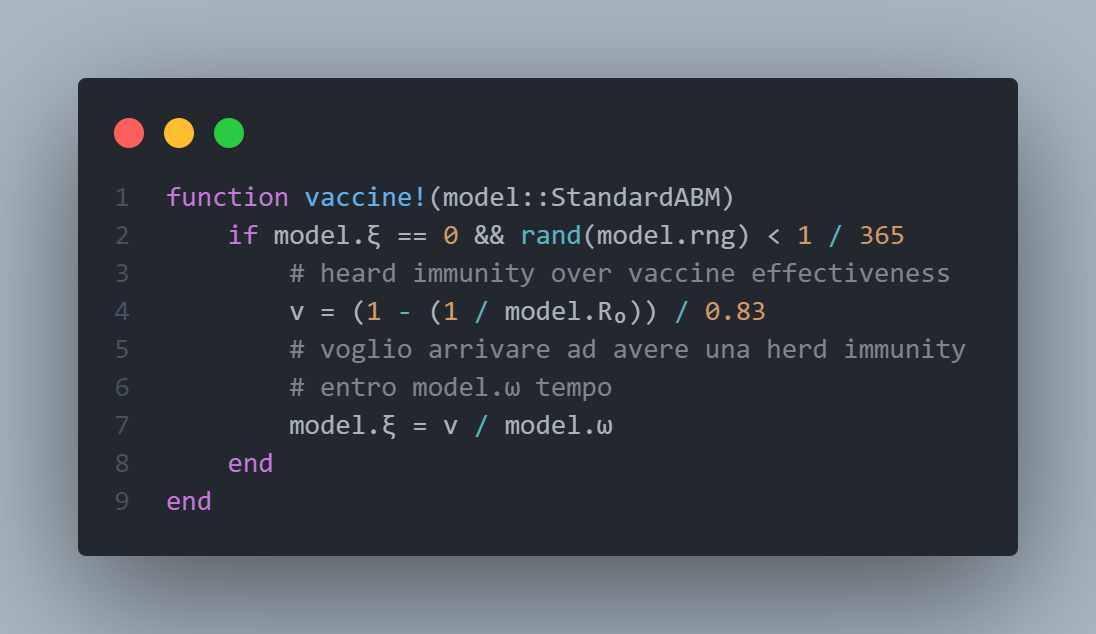
\includegraphics[width=\textwidth]{img/vaccine.png}
	\captionof{figure}{Funzione che si occupa di creare un vaccino}
	\label{fig:vaccine}
\end{minipage}

Questa si occupa di generare il flusso di vaccinazioni giornaliere date dal
calcolo di una \emph{immunita' di gregge} ottenibile tramite un 
percorso vaccinale.\cite{wiki:Immunità_di_gregge}
L'efficacia del vaccino e' stata assegnata seguendo lo studio di meta-analisi \cite{Wu2023-zd}.

Infine la funzione che si occupa di generare la \emph{variant of concern} (VOC) e' la seguente

\begin{minipage}{\linewidth}
	\centering
	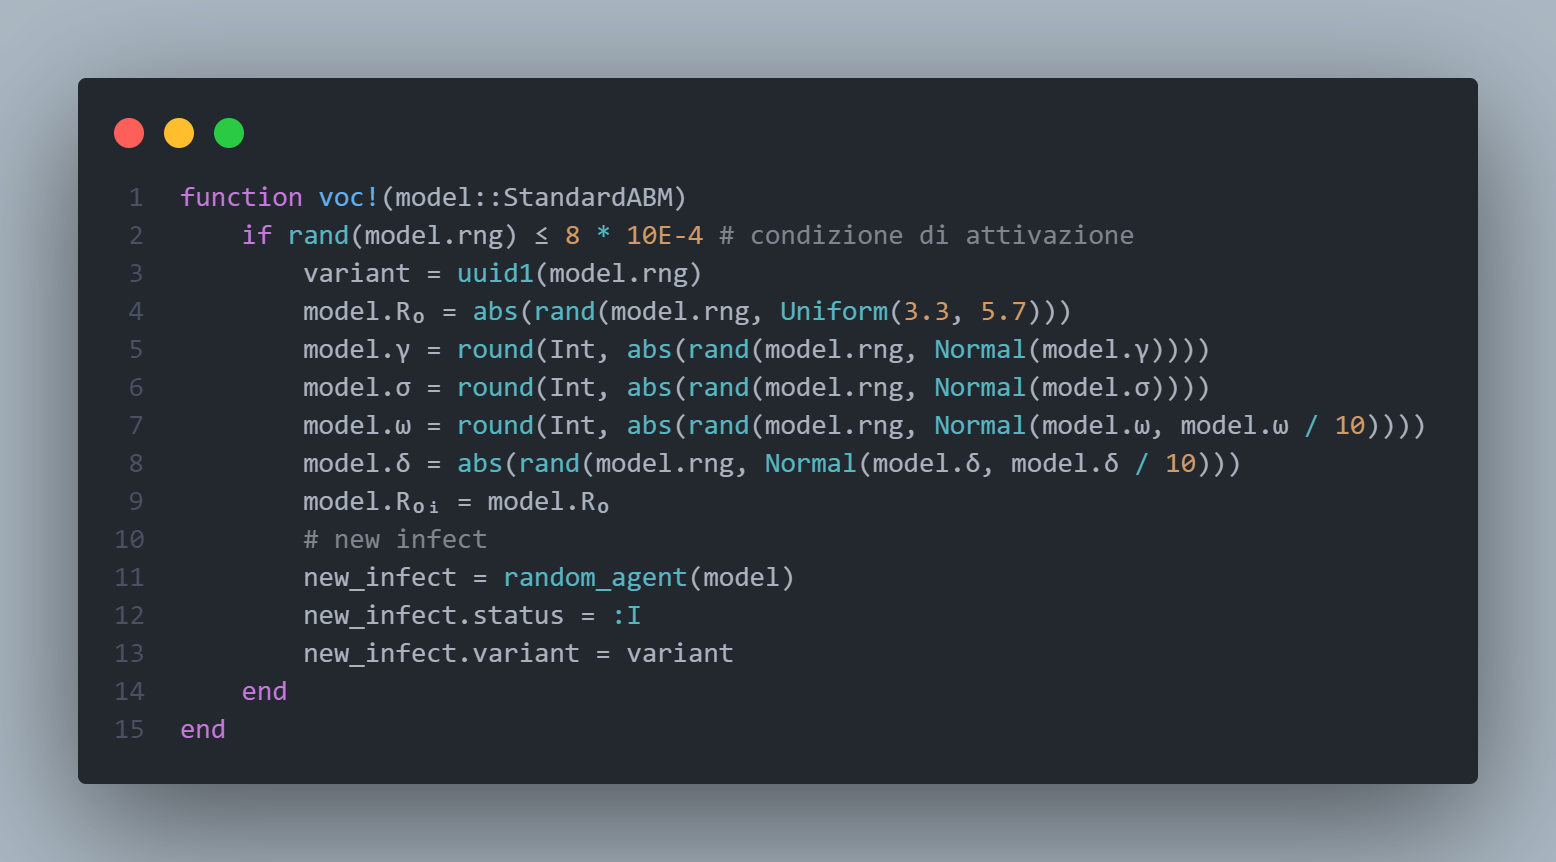
\includegraphics[width=\textwidth]{img/voc.png}
	\captionof{figure}{Funzione che si occupa di generare la VOC}
	\label{fig:voc}
\end{minipage}

Si possono notare molte assunzioni:
\begin{itemize}
	\item la condizione di attivazione della funzione si basa su un valore
	che sembra totalmente randomico. Quel valore, ovvero $8 \cdot 10e-4$ deriva dai
	seguenti articoli \cite{Markov2023} \cite{https://doi.org/10.1002/jmv.27331} \cite{Abavisani2022}
	i quali descrivono prevalentemente il tasso di mutazione casuale delle basi che compongono
	il DNA del virus SARS-COV2. Questo pero' non implica che tali mutazioni 
	creino una VOC. Per semplicita' e' stato scelto di usare l'approccio per cui
	se una mutazione avviene, questa e' un a VOC. In linea di massima sembra che 
	questo approccio semplicistico crei un numero di VOC generalmente sensato e 
	in linea con quanto abbiamo potuto osservare durante la pandemia
	\item la distribuzione dei parametri associati alla pandemia viene calcolata
	seguendo una distribuzione \textbf{Normale}, tranne per la distribuzione dell'indice $R_0$
	il quale segue una distribuzione di tipo \textbf{Uniforme} \cite{wiki:Numero_di_riproduzione_di_base}
\end{itemize}

\subsubsection*{Grafici}

\begin{minipage}{\linewidth}
	\centering
	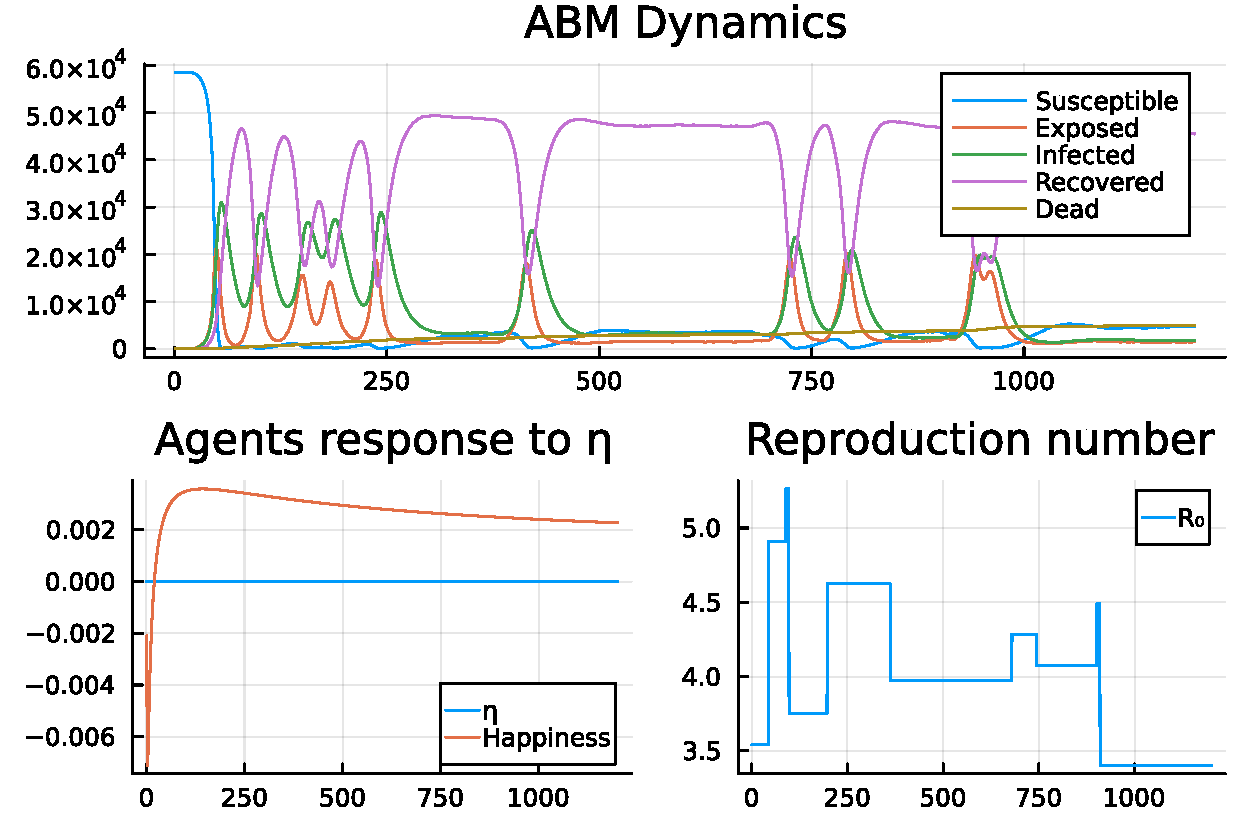
\includegraphics[width=\textwidth]{img/ABM SEIR NO INTERVENTION_2023-06-17.pdf}
	\captionof{figure}{Grafico cumulativo del risultato del modello senza intervento del controllore}
	\label{fig:abm_no_intervent}
\end{minipage}